%%%%%%%%%%%%%%%%%%%%%%%%%%%%%%%%%%%%%%%%%%%%%%%%%%%%%%%%%%%%%%%%%%%%%%%%%%%%%%%%

\section{Model}
\label{sec_model}

V~této kapitole je formalizován model, který popisuje systém těžení a koncept těžebních poolů. Dále je představena strategie sobeckého těžení.

%%%%%%%%%%%%%%%%%%%%%%%%%%%%%%%%%%%%%%%%%%%%%%%%%%%%%%%%%%%%%%%%%%%%%%%%%%%%%%%%

\subsection{Těžení a těžební pooly}
\label{sec_model_mining_and_pools}

Systém je tvořen množinou těžařů $N = 1, \dots, n$. Každý těžař disponuje výpočetním výkonem $p_i$ takovým, že $\sum^n_{i=1} p_i = 1$. Těžař si může vybrat libovolný blok z~blockchainu nad kterým začne těžit. Následující blok vytěží za časový interval, který odpovídá exponenciálnímu rozdělení se střední hodnotou $E(X) = (6 p_i)^{-1}$ hod. Předpis funkce hustoty pravděpodobnosti tohoto rozdělení je zachycen na rovnici~\ref{eq_exp_dist}. Předpokládáme, že těžaři se chovají racionálně -- snaží se maximalizovat svoji odměnu a to i za cenu odchýlení se od protokolu.

\begin{equation}
    f(x)=\left\{\begin{matrix}
        6 p_i \cdot e^{- 6 p_i \cdot x} &; x > 0 \\
        0 &; x \leq 0
    \end{matrix}\right.
    \label{eq_exp_dist}
\end{equation}

\begin{figure}[ht]
    \centering
    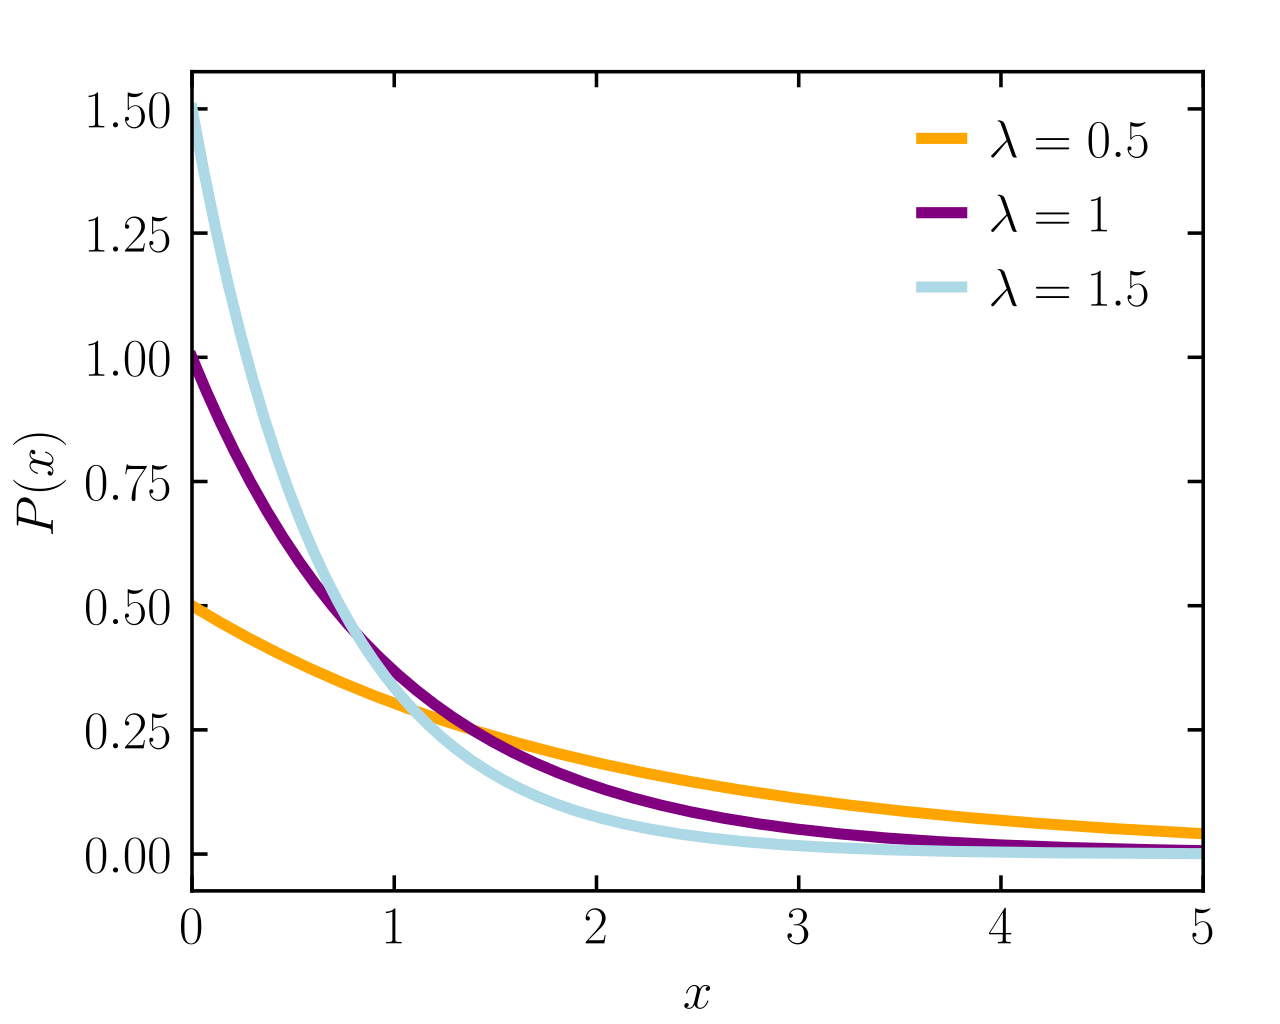
\includegraphics[width=0.625\linewidth]{exponential_probability_density.png}
    \caption{Funkce hustoty pravděpodobnosti pro různá \\
    exponenciální rozdělení ($\lambda = E(X)^{-1} = 6 p_i$).}
    \label{fig_exponential_probability_density}
\end{figure}

Skupina těžařů se může spojit a zformovat tzv. \textit{pool}, který vystupuje v~síti jako jedna entita. \textit{Pool}, který se skládá z~učástníků $M \subseteq N$ disponuje výpočetním výkonem $\sum_{i \in M} p_i \leq 1$. Utržený zisk \textit{pool} rozděluje mezi své členy proporciálně dle jejich výpočetního výkonu. Očekávaný zisk \textit{poolu} je poměr očekávaného počtu vytěžení bloků \textit{poolem} ku celkovému počtu bloků v~nejdelším řetězci. Odměna za vytěžený blok je $R = X + Y$, kde $X$ je počet nově vzniklých bitcoinů a $Y$ je suma všech transakčních poplatků v~bloku. Počet nových bitcoinů za blok se každých $210 000$ vytěžených bloků zmenšuje na polovinu, to v~modelu není nutné zohledňovat.

%%%%%%%%%%%%%%%%%%%%%%%%%%%%%%%%%%%%%%%%%%%%%%%%%%%%%%%%%%%%%%%%%%%%%%%%%%%%%%%%

\subsection{Strategie sobeckého těžení}
\label{sec_model_selfish_mining}

Jak je ukázáno v~kapitole~\ref{sec_analyza}, strategie sobecké těžení (z~anglického \textit{Selfish Mining}) umožňuje těžebnímu aktérovi získat větší odměnu než odpovídá jeho výpočetnímu výkonu. Nezávisí na tom, zda strategii uplatňuje jednolivec či těžební \textit{pool}.

Pro zjednodušení uvažujme rozdělení těžebních aktérů do dvou skupin. Jedna skupina jako $pool$ S~se strategií sobeckého těžení, který disponuje minoritním výpočetním výkonem ($p_S < 0,5$). A~zbytek sítě jako skupinu poctivých těžařů (\textit{honest miners}) s~ostatním  výpočetním výkonem ($1 - p_S$). Není podstatné, zda zbytek figuruje jako jedna entita, nebo několik menších skupin.

Podstata sobeckého těžení spočívá v~přimětí poctivých těžařů ke zbytečnému těžení. Spotřebovávání zdrojů na aktivitu, za kterou nebudou odměněni. Konkrétně způsobit, že poctiví těžaři budou těžit takovou větev blockchainu, která ve výsledku nebude součástí nejdelšího řetězce. Taková situace může nastat i ve standardních podmínkách, kdy se všichni chovají poctivě, avšak strategie sobeckého těžení bude způsobovat, že poctiví těžaři budou takové situaci vystaveni častěji.

Sobečtí těžaři tohoto cíle dosahují specifickou strategií odhalování jimi vytěžených bloků. Pokud \textit{pool} S~vytěží blok výšky $n$, nepošle ho do sítě ostatním ihned, nýbrž si ho nechá pro sebe a blok $n + 1$ těží sám. Disponuje tak nejdelším řetězcem, o~kterém nikdo další neví. Zbytek sítě dále pokračuje na veřejné větvi blockchainu a těží blok $n$. Situace se dále může vyvíjet různě, avšak jelikož \textit{pool} S~disponuje pouze minoritou výpočetního vykonu, jeho soukromá větev blockchainu nebude nejdelší do nekonečna. \textit{Pool} S~s~tím kalkuluje a uvážlivě odhaluje bloky ze své soukromé větve tak, aby způsoboval, že poctiví těžaři opustí veřejnou kratší větev, nad kterou nějaký čas těžili. To znamená že investovali výpočetní výkon zbytečně.

Se znalostí této intuice je možné plně specifikovat algoritmus sobeckého těžení.

\bigskip
\begin{lstlisting}[
    language = myLang,
    caption={Algoritmus sobeckého těžení -- inicializační fáze.}
]
public chain = publicly known blocks
private chain = publicly known blocks
privateBranchLenght = 0
do: Mine at the head of the private chain
\end{lstlisting}

\bigskip
\begin{lstlisting}[
    language = myLang,
    caption = {Algoritmus sobeckého těžení -- situace, kdy sobecký \textit{pool} vytěžil blok.}
]
diff = length(private chain) - length(public chain)
append new block to the private chain
privateBranchLenght += 1

// selfish pool wins due to the lead of 1
if diff == 0 and privateBranchLenght == 2:
    do: publish all the private chain
    privateBranchLenght = 0

do: Mine at the head of the private chain
\end{lstlisting}

\bigskip
\begin{lstlisting}[
    language = myLang,
    caption = {Algoritmus sobeckého těžení -- situace, kdy zbytek sítě vytěžil blok.}
]
diff = length(private chain) - length(public chain)
do: append the new block to the public chain

// they win
if diff == 0:
    private chain = public chain
    privateBranchLenght = 0

// now it's the same length, luck decides
else if diff = 1:
    do: publish last block of the private chain

// selfish pool wins due to the lead of 1
else if diff = 2:
    do: publish all the private chain
    privateBranchLenght = 0

// diff > 2
else:
    do: publish first unpublished block in private block

do: Mine at the head of the private chain
\end{lstlisting}
\bigskip

Strategie je řízena těžebními událostmi v~síti. Rozhodnutí sobeckého \textit{poolu} závisí na rozdílu délek privátní a veřejné větve blockchainu. V~následujících odstavcích je chování sobeckého těžaře popsáno v~konkrétních situací.

Veřejná vetěv blockchainu je delší než soukromá větev sobeckého \textit{poolu}. V~tomto případě sobecký pool přijme nový blok vytěžený zbytkem sítě a začne těžit nad ním. Vzhledem k~distribuci výpočetního výkonu bude tato situace nastávat nejčastěji.

Sobecký těžař vytěží blok a má náskok jednoho bloku nad veřejným blockchainem. Místo toho, aby ho naivně ihned zveřejnil a poslal do sítě, si ho nechá pro sebe a těží nad ním sám. Následovat mohou dvě situace.

Další blok vytěží zbytek sítě, v~tomto případě nastává \textit{fork} blockchainu a následně hraje klíčovou roli latence mezi jednotlivými uzly. V~momentě, kdy se informace o~nově vytěženém bloku někým dalším dostane k~sobeckému těžaři, ihned zveřejní svůj již dřívě vytěžený blok. V~tuto chvíli nastává dočasná nekonzistence mezi uzly v~síti. Část sítě těží nad blokem vytěženým sobeckým těžařem a část nad blokem vytěženým zbytkem sítě. Kdo vytěží další blok vyhrál, má nejdelší blockchain a zbytek sítě akceptuje jeho verzi.

Pokud další blok vytěží opět sobecký těžař, dosahuje pohodlného náskoku dvou bloků. V~takovém případě sobecký pool pokračuje dále v~těžení nad svojí větví blockchainu. Další blok zveřejní vždy, pokud zbytek sítě vytěží blok na veřejné větvi a tím sníží jeho náskok. Jelikož sobecký pool má minoritní výpočetní výkon, v~určitém bodě bude jeho náskok snížen natolik, že zveřejní svoji soukromou větev celou. Jelikož jeho větev je nejdelší, zbytek sítě ji akceptuje. Sobecký pool získá odměnu všech bloků ve své větvi, zatímco zbytek sítě spotřebovával elektřinu zbytečně.

%%%%%%%%%%%%%%%%%%%%%%%%%%%%%%%%%%%%%%%%%%%%%%%%%%%%%%%%%%%%%%%%%%%%%%%%%%%%%%%%
